\documentclass[a4paper,11pt]{article}
\usepackage{polski}
\usepackage[utf8]{inputenc}
\usepackage{graphicx}
\pagestyle{empty}
\title {Symulator tomografu komputerowego}
\author{Mateusz Urbaniak, 127345 \and Filip Błaszczyk, 127316}
\begin{document}
\maketitle

\section{Wstęp}
Zadany problem stworzenia symulatora tomografu komputerowego, zrealizowaliśmy poprzez napisanie algorytmu w języku Java, oraz przedstawienie wyników w interfejsie graficznym napisanym w języku JavaFX. Przeprowadziliśmy filtrację sinogramu, pominęliśmy filtrację zrekonsturowanego obrazu (gdybyśmy ponownie realizowali projekt, skupilibyśmy się na wykorzystaniu Pythona i bibliotek numpy i innych, które ułatwiłyby nam przeprowadzenie Transformacji i Odwrotnej Transformacji Fouriera (mieliśmy problemy z własną implementacją w Javie). Wybraliśmy model stożkowy układu emiter-detektory.

\section{GUI}
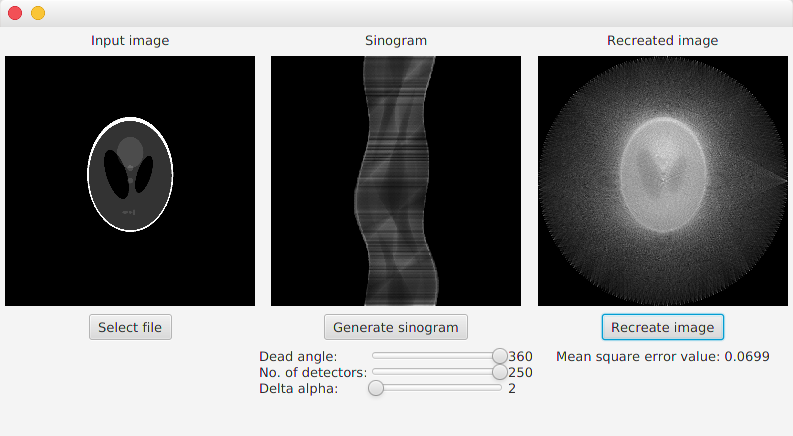
\includegraphics[width=\textwidth]{GUI}
Ładujemy obraz do przetwarzania poprzez przycisk "Select file".
Następnie ustawiamy parametry "Dead angle" (rozwartość układu emiter-detektory), "No. of detectors" (ilość detektorów) oraz "Delta alpha" (wpływające na ilość iteracji w obrębie od 0 do 360 stopni). Następnie generujemy sinogram poprzez kliknięcie w przycisk "Generate sinogram". Po wygenerowaniu sinogramu, klikamy w przycisk "Recreate image" aby odtworzyć nad podstawie sinogramu obraz wejściowy. Pod tym przyciskiem znajduje się informacja o wartości błędu średniokwadratowego (suma kwadratów różnic między obrazem wejściowym a obrazem zrekonstruowanym, podzielona przez rozmiar obrazu wejściowego).

\section{Wykresy}
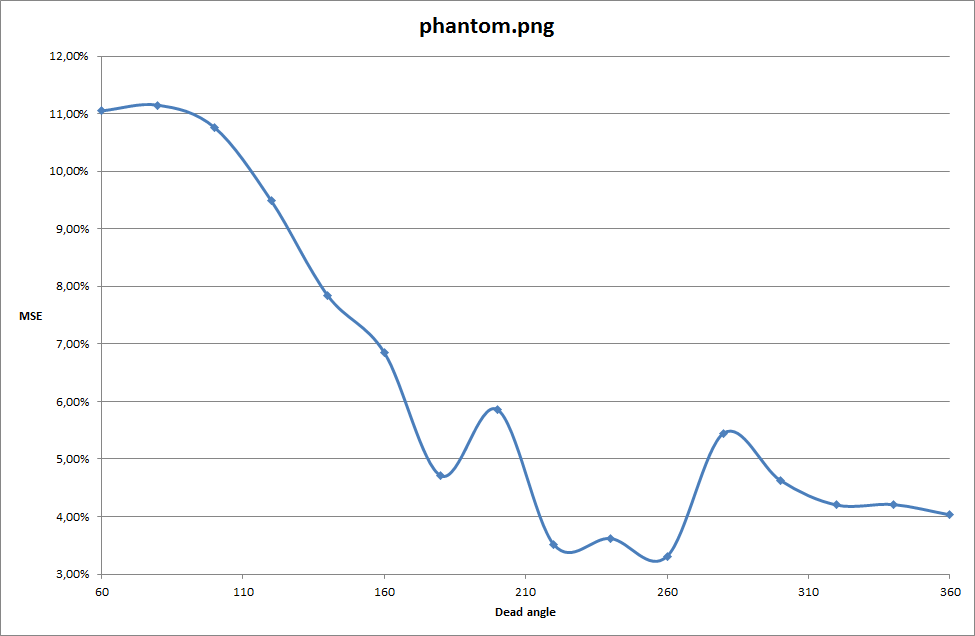
\includegraphics[width=\textwidth]{phantomDeadAngle}
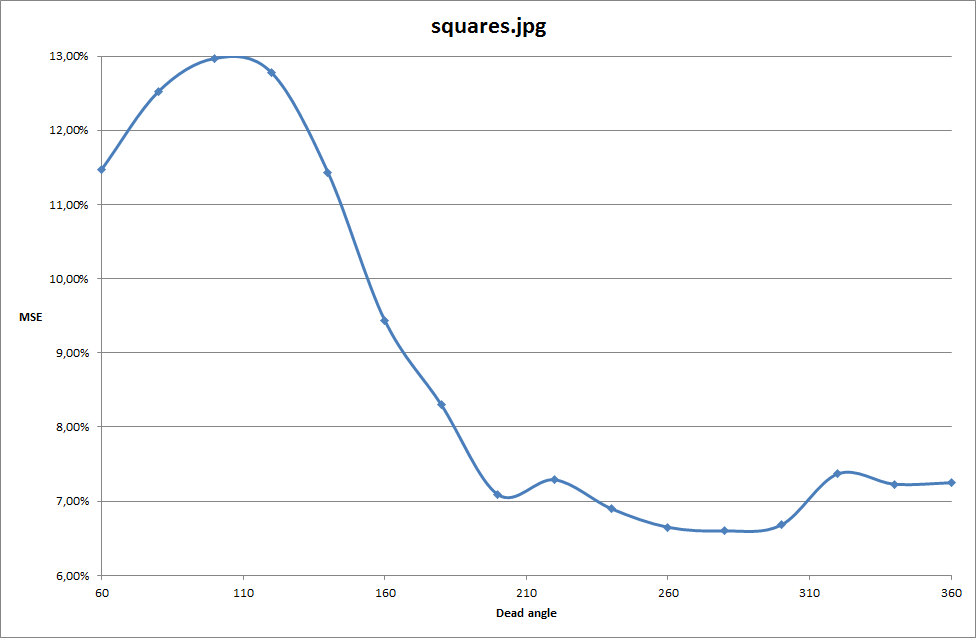
\includegraphics[width=\textwidth]{squaresDeadAngle}
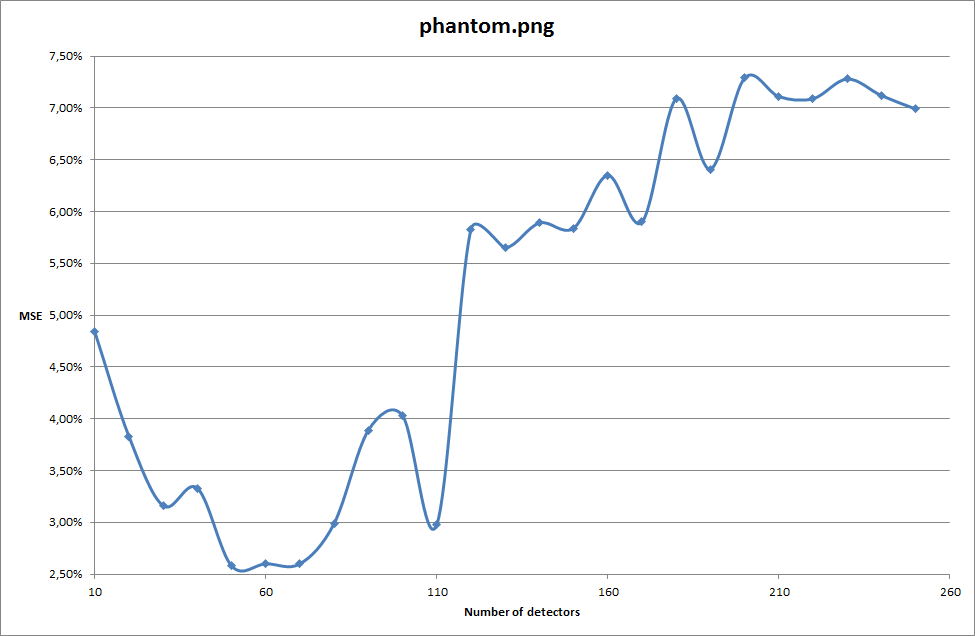
\includegraphics[width=\textwidth]{phantomDetectors}
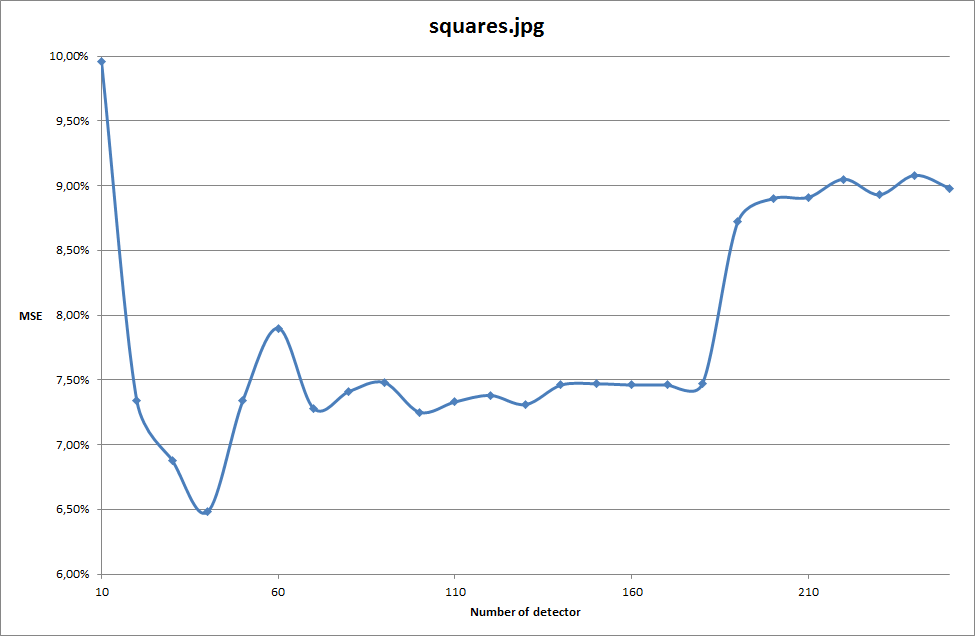
\includegraphics[width=\textwidth]{squaresDetectors}
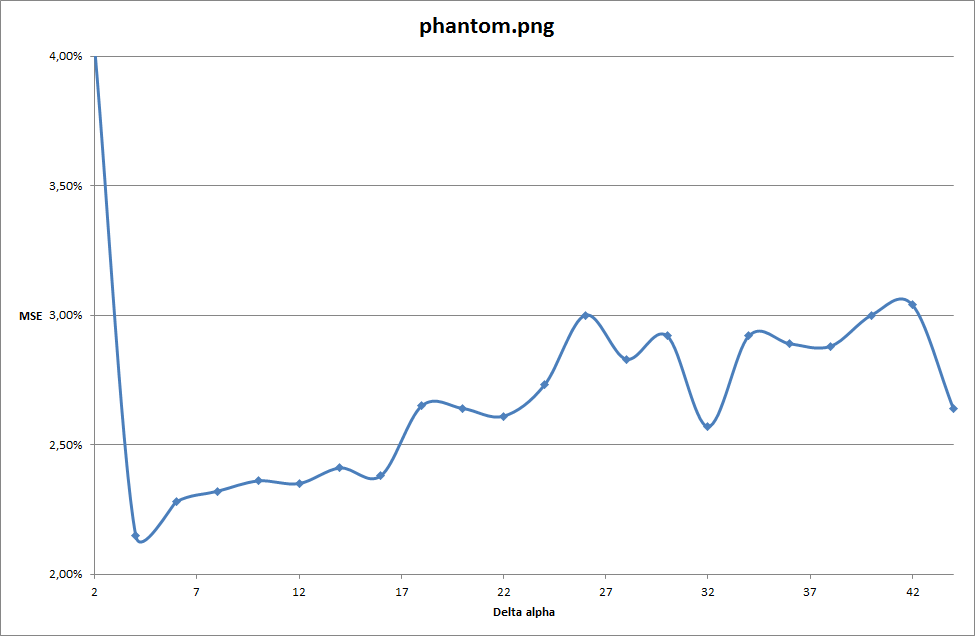
\includegraphics[width=\textwidth]{phantomAlpha}
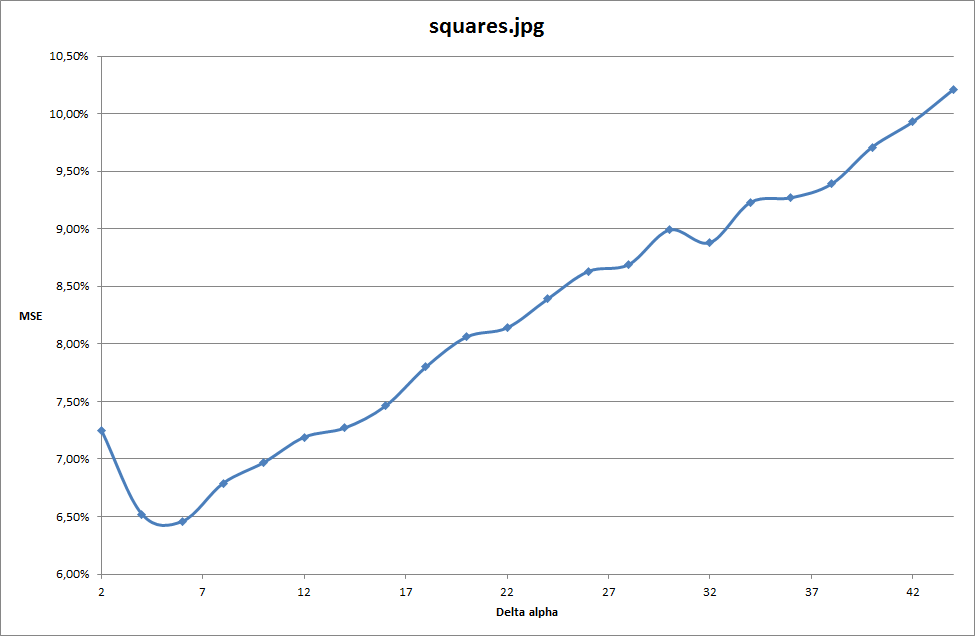
\includegraphics[width=\textwidth]{squaresAlpha}

\section{Wnioski}
MSE - Mean Square Error (błąd średniokwadratowy)\\\\
Zwiększanie rozwartości układu emiter-dekodery, w perspektywie długofalowej zmniejszało MSE i czyniło obraz bardziej podobnym do obrazu wejściowego.\\
Zwiększanie liczby detektorów zwiększało MSE, które jednak nie miało odzwierciedlenia w podobieństwie obrazu odtworzonego do obrazu wejściowego - ten wraz ze zwiększaniem liczby detektorów, był wierniejszym odtworzeniem obrazu wejściowego.\\
Zwiększanie wartości delta alpha (a przy tym zmniejszanie ilości iteracji generowania sinogramu i odtwarzania obrazu) powodowało zwiększenie MSE i zmniejszało podobieństwo obrazu odtworzonego do obrazu wejściowego.
\end{document}